\section{Motivation}\label{sec:motivation}
We first designed and experimented with three simple graph index update methods, and compared them with the most advanced dynamic graph index FreshDiskAnn\cite{DBLP:journals/corr/abs-2105-09613}. After an in-depth analysis of the reasons why these methods did not perform well, we proposed our own graph index deletion algorithm.
\subsection{Experimental methods}
%我们首先设计实验以验证更新算法的有效性。在此之前我们先回顾我们对动态ANN搜索算法的三个目标:在更新前后大小相同且数据分布相似的数据集上,动态ANNS算法需要达到以下三个条件:(1)图索引精度不下降或下降很少,(2)搜索吞吐量不下降或下降很少,(3)更新速度足够快。我们的实验也将关于这三个条件来设计。
We first design experiments to verify the effectiveness of an updating algorithm. Before that, let us review our three goals for the dynamic ANN search algorithm: on datasets of the same size and similar data distribution before and after the update, the dynamic ANN search algorithm needs to meet the following three conditions: (1) the graph index accuracy does not decrease or decreases very little, (2) the search throughput does not decrease or decreases very little, and (3) the update speed is fast enough. Our experiments will also be designed with these three conditions in mind.

%为保证数据集大小相同且数据分布相似,我们首先在数据集中随机选择一部分点删除,随后再将这些点插入到数据集中,并观察更新前后,图索引对于相同查询的查询精度变化以及各项操作的吞吐量变化。由于更新前后数据集未发生变化,所以对于一个有效的动态ANNS算法,应该能在该实验中满足我们提出的三个条件。为观察更新操作对图索引的持续影响,我们将该过程重复多次,并观察每个周期中图索引各项指标的变化情况。
To ensure that the data sets are of the same size and have similar data distribution, we first randomly select a portion of points in the data set to delete, and then insert these points into the data set, and observe the changes in the query accuracy of the graph index for the same query and the throughput of various operations before and after the update. Since the data set does not change before and after the update, an effective dynamic ANNS algorithm should be able to meet the three conditions we proposed in this experiment. To observe the continuous impact of the update operation on the graph index, we repeated the process multiple times and observed the changes in various indicators of the graph index in each cycle.

\subsection{Simple deletion method}
We conducted experiments based on two widely used ANNS algorithms, HNSW and FreshDiskAnn, of which FreshDiskAnn uses its memory version. HNSW is a graph index algorithm designed based on SNG graph, while FreshDiskAnn is a graph index algorithm designed based on a variant of SNG graph, namely $\alpha$-RNG, which relaxes the edge selection condition of SNG to make it suitable for update operations. Among them, FreshDiskAnn can support both insertion and deletion operations, while HNSW only supports insertion, so we implemented the following three simple deletion strategies in HNSW. Due to the multi-layer structure of HNSW, when deleting any point, we delete the point from each layer in HNSW:

\paragraph{\textbf{The violent deletion strategy}} deletes only the outgoing and incoming edges of the deleted point when deleting the point $p$, and does not add any additional edges to compensate for the lack of connectivity caused by the deletion.

\paragraph{\textbf{Fully connected deletion strategy}}After deleting the outgoing and incoming edges of point $p$, add edges to the neighborhood of point $p$: if there are edges $(p_{in},p)$ and edges $(p,p_{out})$, add edge $(p_{in},p_{out})$ to $p_{in}$, and execute the edge pruning algorithm for points $p_{in}$ that exceed the degree limit to strictly limit the out-degree of each point to less than the out-degree upper limit $R$. It is worth noting that this method is also the deletion strategy used by FreshDiskAnn.

\paragraph{\textbf{Re-search deletion strategy}}After deleting the outgoing and incoming edges of point $p$, add edges to the neighborhood of point $p$: for all points $p_{out}$, use $GreedySearch(\mathbf{G},\mathbf{G}.s,p_{out},L,L)$ to obtain the candidate set $C$, and then use $LinkSelect(p_{out},C,D)$ to filter out $D$ points from the candidate set. For each point in the filter result, add an edge pointing to the current $p_{out}$. For points with out-degree exceeding $R$, use $LinkSelect$ to limit their out-degree to $R$.

%我们在128维的sift1M数据集上进行了实验,每次循环随机选取其中5%的点进行更新,并将所有实验的线程数设为64线程。我们设置HNSW的参数为$M=32,ef=200$,FreshDiskAnn的映射参数为$R =32,L=200$,搜索参数为$L=100$。由于我们对两个算法的参数设置相同,因此HNSW和FreshDiskAnn的初始索引的召回率100-recall@100仅相差0.0075,FreshDiskAnn的初始索引略高于HNSW。暴力删除策略和全连接删除策略不需要设置参数,重新搜索删除策略的参数设置为$D=32$。实验结果如图\ref{SamplePolicy}所示。
We conducted experiments on the 128-dimensional sift1M dataset, randomly selecting 5\% of the points for update in each cycle, and set the number of threads for all experiments to 64 threads. We set the parameters of HNSW to $M=32, ef=200$, the mapping parameters of FreshDiskAnn to $R=32, L=200$, and the search parameter $L=100$. Since we set the same parameters for the two algorithms, the recall rate 100-recall@100 of the initial index of HNSW and FreshDiskAnn differs by only 0.0075, and the initial index of FreshDiskAnn is slightly higher than that of HNSW. The violent deletion strategy and the fully connected deletion strategy do not need to set parameters, and the parameter of the re-search deletion strategy is set to $D=32$. The experimental results are shown in Figure \ref{SamplePolicy}.

\begin{figure}[h]
	\centering
	\begin{minipage}{0.49\linewidth}
		\centering
		\vspace{3pt}
		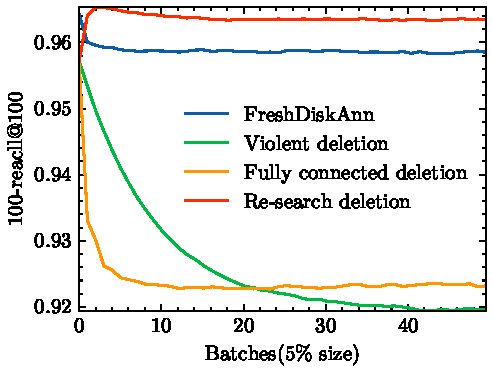
\includegraphics[width=\textwidth]{fig/Result/SIFT1M/SamplePolicy_FreshDiskAnn_recall.pdf}
	\end{minipage}
	\begin{minipage}{0.49\linewidth}
		\centering
		\vspace{3pt}
		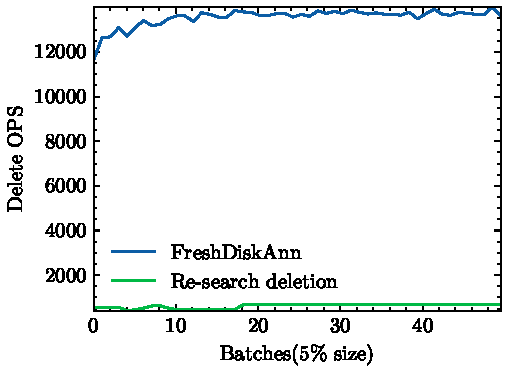
\includegraphics[width=\textwidth]{fig/Result/SIFT1M/SamplePolicy__delete_OPS.pdf}
	\end{minipage}
	\caption{Search recall over 20 epochs using statically constructed HNSW and Vamana to delete and reinsert 5\% of the SIFT1M dataset. The parameters of HNSW are set to $\mathbf{M=32, ef=200}$, the parameters of FreshDiskAnn are set to $\mathbf{R=32, L=200}$, and the search parameters are set to $\mathbf{Ls=100}$. The parameters of the re-search deletion strategy are set to $\mathbf{D=32}$.}
	\label{SamplePolicy}
\end{figure}

From the above experimental results, it can be seen that only the update methods of re-search deletion strategy and FreshDiskAnn can ensure that the query accuracy does not decrease or decreases very little. Among them, although FreshDiskAnn finally stabilizes at a higher accuracy, it also has a decrease in accuracy in the first few cycles, while the accuracy of the re-search deletion strategy increases rapidly with the update and remains at a high accuracy. The other two simple deletion strategies will cause a sharp drop in query accuracy. However, in the right figure of \ref{SamplePolicy}, we can see that the deletion throughput of the re-search deletion strategy is much lower than that of FreshDiskAnn. The deletion throughput of the re-search deletion strategy is only maintained at 680 deletions per second, while that of FreshDiskAnn is 13,800 deletions per second. Such a throughput is obviously difficult to meet our design goals.

\subsection{Reasons for poor performance}
We first analyze the reasons why the accuracy of the brute force deletion strategy and the full connection deletion strategy decreases after the update. We believe that the main reason for this phenomenon is that the deletion operation in MSNET destroys the monotone path. Since the deleted points are likely to be points on multiple monotone paths in the graph, this will cause the monotone path to be destroyed, thereby reducing the index accuracy. Moreover, since the existing graph indexes are designed using approximate neighbor graphs, these approximate neighbor graphs cannot guarantee that there is a monotone path between each pair of points, so the impact of monotone path destruction will be greater than that of the accurate neighbor graph.

Taking the case in the figure \ref{MSNET_delete} as an example, in an approximate SNG graph, point $s$ is the search starting point, and there is only one monotone path $MP(p_{in},p_{out})$ from point $p_{in}$ to point $p_{out}$, that is, $p_{in}, p, p_{out}$. When the violent deletion strategy is used to delete point $p$, all monotone paths passing through point $p$ (i.e., $MP(s,p_{out})$ and $MP(s,q)$) are destroyed, resulting in a decrease in the accuracy of the graph index. When the fully connected deletion strategy is used to delete point $p$, since $\delta(p_{in},r)<\delta(p_{in},p_{out})$, point $r$ will be preferentially selected as the outer neighbor of point $p_{in}$. After selecting point $r$, since $\delta(r,p_{out})<\delta(p_{in},p_{out})$, point $p_{out}$ will be excluded from the candidate set, so the edge $\overrightarrow{p_{in},p_{out}}$ cannot be connected, and the monotone paths $MP(s,p_{out})$ and $MP(s,q)$ cannot be restored. Although FreshVamana alleviates this phenomenon by relaxing the edge cutting condition, making the edge $\overrightarrow{p_{in},p_{out}}$ more likely to be connected when the situation shown in the figure \ref{MSNET_delete} occurs, it still does not completely solve the problem of monotone path destruction, which causes the problem of reduced accuracy in the first few cycles.

\begin{figure}[h]
	\centering
	\begin{minipage}{0.49\linewidth}
		\centering
		\vspace{3pt}
		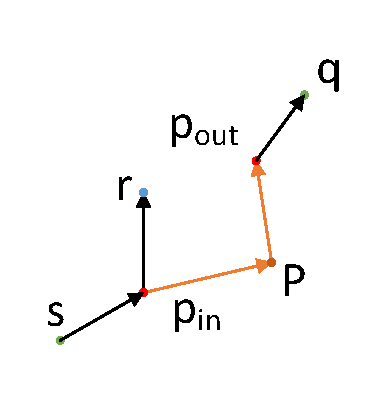
\includegraphics[width=\textwidth]{fig/Example/MSNET_delete_before.pdf}
		Before deleting point p
	\end{minipage}
	\begin{minipage}{0.49\linewidth}
		\centering
		\vspace{3pt}
		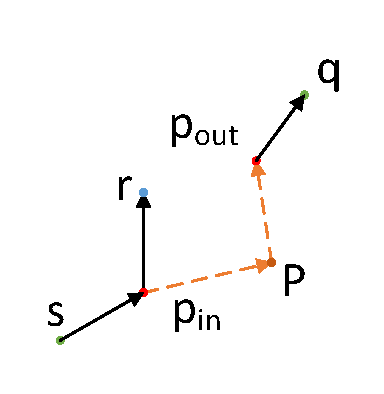
\includegraphics[width=\textwidth]{fig/Example/MSNET_delete_policyA.pdf}
		The violent deletion strategy
	\end{minipage}
	\begin{minipage}{0.49\linewidth}
		\centering
		\vspace{3pt}
		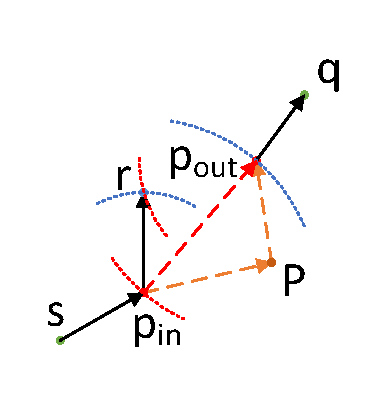
\includegraphics[width=\textwidth]{fig/Example/MSNET_delete_policyB.pdf}
		Full connection deletion strategy
	\end{minipage}
	\begin{minipage}{0.49\linewidth}
		\centering
		\vspace{3pt}
		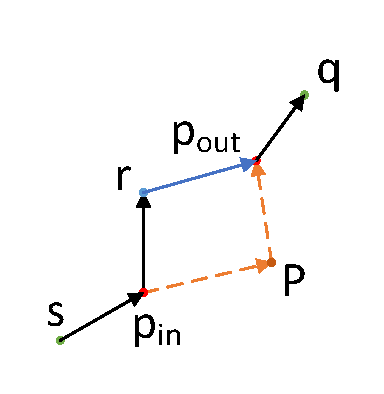
\includegraphics[width=\textwidth]{fig/Example/MSNET_delete_policyC.pdf}
		Re-search deletion strategy
	\end{minipage}
	\caption{This figure is an approximate SNG graph, where point $s$ is the search starting point. The four figures show the situation before and after point $p$ is deleted using different deletion strategies.}
	\label{MSNET_delete}
\end{figure}

The reduction in accuracy caused by the deletion operation makes it difficult to obtain an accurate candidate set when reinserting. This means that although we reinsert the deleted points into the dataset, the reinserted points cannot accurately restore their connectivity due to the inaccurate candidate set. Therefore, the index accuracy decreases after each cycle.

Unlike the previous two deletion strategies, the re-search deletion strategy works well in terms of graph index accuracy, and even after the update, the graph index accuracy is improved. This is mainly because the Re-search deletion strategy re-searches the candidate set of the outer neighbors of the point $p_{out}$ and connects the more reasonable points around the point $p_{out}$ to $p_{out}$. Taking the case in figure \ref{MSNET_delete} as an example, after deleting point $p$ and its related edges, searching for points around point $p_{out}$ as a candidate set can find point $r$. After connecting point $r$ to point $p_{out}$, not only the monotone path $MP(s,p_{out })$ is restored, but also since edge $\overrightarrow{r,p_{out}}$ is also monotone to point $q$, $MP(s,q)$ can also be repaired. Considering that we obtain multiple candidate points through search and filter the candidate points through the SNG edge trimming algorithm, the edges finally connected to point $p_{out}$ will evenly come from multiple directions, so these edges are likely to be monotone to the endpoints of the monotone paths that passed through the edge $\overrightarrow{p,p_{out}}$ before deletion, so these monotone paths can also be repaired. Moreover, since the deletion algorithm effectively restores the monotone path $MP(s,p_{out })$, when the deleted point is inserted again, the insertion algorithm can search for a more accurate candidate set, improving the accuracy of updating the graph index.

However, each time each point $p_{out}$ is deleted, the external neighbor candidate set must be searched again, which takes too long and is difficult to meet our requirements for deletion efficiency.

Based on the above analysis, designing a fast and effective deletion algorithm is the key to the graph index update algorithm. We need to quickly find those points that can repair the monotone path $MP(s,p_{out})$ and connect them to the point $p_{out}$ to repair the monotone path $MP(s,p_{out})$.



